\documentclass[14pt,a4paper,final]{extreport}
\usepackage[utf8]{inputenc}
\usepackage{amsmath}
\usepackage{amsfonts}
\usepackage{enumerate}
\usepackage{enumitem}
\usepackage{amssymb}
\usepackage[colorlinks]{hyperref}
\usepackage{graphicx}
\usepackage[left=3cm,right=2cm,top=2cm,bottom=2.5cm]{geometry}
\linespread{1.2}
\usepackage{titlesec}
\usepackage[utf8]{inputenc}
\usepackage[english]{babel}
\usepackage{fancyhdr}
\usepackage{soul}
\usepackage{ulem}
\usepackage{xcolor}
\usepackage{array, xcolor, lipsum, bibentry,fancyhdr}
\usepackage[margin=3cm]{geometry}

\usepackage{etoolbox}
\patchcmd{\chapter}{\thispagestyle{plain}}{\thispagestyle{fancy}}{}{}

\let\cleardoublepage\clearpage
%to remove the dots for the content page.
\makeatletter
\renewcommand{\@dotsep}{10000} 
\makeatother
\makeatletter 
%\renewcommand{\thefigure}{\@arabic\c@figure}
\makeatother




\definecolor{lightgray}{gray}{0.8}
\newcolumntype{L}{>{\raggedleft}p{0.14\textwidth}}
\newcolumntype{R}{p{0.8\textwidth}}
\newcommand\VRule{\color{lightgray}\vrule width 0.5pt}
%....................................
%....................................
%change this portion in ur tex file. copy this and paste there.
%....................................
%....................................

\titleformat{\chapter}[display]
{\normalfont\rmfamily\medium\bfseries\color{black}}
{\chaptertitlename\ \thechapter}{13pt}{\LARGE}
 
\titlespacing {\chapter}{0pc}{0pc}{.1pc}
%\titlespacing{<command>}{<left>}{<before-sep>}{<aft

\titlespacing{\section}{0pc}{.5pc}{0pc}
\titlespacing{\subsection}{0pc}{1pc}{0pc}


%........................................
%........................................
%thank u
%........................................
%........................................

\author{{{by}}\\
\textbf{VIVEK E }\\
	(Roll No:31)\\[2pt]
 }
\title{{\large\textbf{AMMINI COLLEGE OF ENGINEERING PALAKKAD}} \\
\begin{figure}[h]
	\begin{center}

\includegraphics[scale=.6]{images.jpg} \\[.1cm]
\end{center}
\end{figure}
{\large\textbf{SEVENTH SEMESTER B.TECH\\[.5 cm]}}
	{\large\textbf{SEMINAR REPORT\\[.5 cm]}}
	{\large \textbf{ON\\[.2 cm]}}
	{\large \textbf {PROGRESSIVE WEB APPS}}
		}
\date{
\textit{under the guidance of} \\[0.2cm]
	\textbf{ Mr. Sudhesh K.M} \\
	\textbf{Assistant Professor}\\
	\vspace{.1cm}
	\large\textbf{Department of Computer Science and Engineering} \\
}	
\thispagestyle{empty}

\begin{document}
\pagenumbering{gobble}
\clearpage\maketitle
\thispagestyle{empty}


\begin{center}\fontsize{17}{17} \selectfont \textbf{AMMINI COLLEGE OF ENGINEERING PALAKKAD}\end{center}
%\begin{center}\fontsize{14}{17} \selectfont \textbf{PALAKKAD}\end{center}
\begin{figure}[h]
	\begin{center}
		
\includegraphics[scale=.7]{images.jpg}
		\vspace{.1 cm}
	\end{center}
\end{figure}
\begin{center}\fontsize{17}{17} \selectfont \textbf{\large Department of Computer Science \& Engineering\\[2cm] }\end{center}
\begin{center}
\emph{\textcolor{red}{\Large \bf CERTIFICATE}}
\end{center}
{This is to certify that the seminar report entitled {\bf{PROGRESSIVE WEB APPS}} submitted by {\bf VIVEK E}, to the {\bf Department of Computer Science and Engineering, Ammini College of Engineering, Palakkad -678613}, in partial fulfilment of the requirement for the award of B.Tech Degree in Computer Science and Engineering is a bonafide record of the work carried out by him.}
\newline
\newline
\newline
\newline
  \hspace{1cm}Mr Sudhesh K M\hspace{8.7cm}Mr Prabhu M
\newline
Co-ordinator \& Guide\hspace{6.75cm} Head Of Department
\newline
\newline
Place$:$\hspace{.5cm}Palakkad 
\newline
\renewcommand{\dateseparator}{-}
Date$:$\hspace{.5cm}\date{25-10-2019}%13-09-2010
\newline


%\thispagestyle{empty}

\newpage
\section*{\begin{center} \fontsize{14}{17} \selectfont \textbf{Acknowledgement}\end{center}}
\thispagestyle{empty}
%\vspace{1cm}

%\vspace{.4 cm }
%\begin{quote}
{                                                 
	\hspace{01.5cm}It is with great enthusiasm and learning spirit that I am bringing out this seminar report. Here I would like to mark my token of gratitude to all those who influenced me during the period of my work. I would like to express my sincere thanks to \textbf{The Management of Ammini College of Engineering, Palakkad} and \textbf{Dr.Suresh Kumar V }, The Principal Ammini College of Engineering for the facilities provided here.
\par
	\hspace{01.5cm}I express my heart-felt gratitude to Head of the Department, \textbf{Mr. Prabhu M} , Assistant Professor Department of Computer Science \& Engineering for allowing me to take up this work.
\par	
	\hspace{01.5cm}With immense pleasure I express sincere thanks to my guide and   Co-Ordinator \textbf{Mr. Sudhesh K.M} , Assistant Professor for his committed guidance, valuable suggestions and constructive criticisms. His stimulating suggestions and encouragement helped me through my seminar work. I extend my gratitude to all teachers in the Department of Computer Science and Engineering, Ammini College of Engineering, Palakkad for their support and inspiration.
\par
	\hspace{01.5cm}And above all I praise and thank the Almighty God, who showered His abundant grace on me to make this seminar a success. I also express my special thanks and gratitude to my family and all my friends for their support and encouragement.
}
%\end{quote}
%header footer....
\pagestyle{fancy}
\lfoot{{\tiny AMMINI COLLEGE OF ENGINEERING}}
\chead{}
\rfoot{\tiny{DEPT OF CSE}}
\rhead{\tiny \thepage}
\cfoot{}
\lhead{\tiny{PROGRESSIVE WEB APPS}}
\renewcommand{\headrulewidth}{0.6pt}
\renewcommand{\footrulewidth}{0.6pt}
\newpage
\textbf{
\begin{center}
\abstractname{}
\thispagestyle{empty}
\end{center}}
The mobile apps have been reaching a huge success on the mobile market. This
opportunity attracted a lot of interested companies to have their own optimized mobile
apps for all major mobile operation systems. However, these developments are expensive
when developed natively for each mobile platform. New improvements done on the web
technologies, allowed more features and capabilities than previously was only possible on
apps that was developed natively. This started new possibilities on consolidate all
developments only on web apps, that are apps that runs on web browsers. Progressive
apps load quickly even on slow network connections, send push notifications, and have a
splash screen and an icon on the home screen. When launched from the home screen,
these apps blend into the environment; they’re top-level, full-screen, and work offline.
Progressive web apps are an interesting forward look into the future of mobile apps.

 




\tableofcontents % compile 2 times to get table of contents written
\addtocontents{toc}{\small}


\listoffigures  %compile 2 times to get list of figures written
\addtocontents{lof}{\small}


\clearpage
\pagenumbering{arabic}
\chapter{Introduction}
The mobile Web is becoming ever more capable of accessing and handling features previously only available in native and cross-platform apps. With the introduction of Progressive Web Apps (PWAs), regular Web sites can to a larger extent than before act, feel and look as any other installed app – so far particularly on an Android- based mobile device. This is enabled through a set of new concepts and requirements, advocated by Google as well-worth implementation efforts. In short, a PWA is any Web site implementing certain specific technical features. Such a Web site can, in PWA-supported browsers, be added to the home-screen of a user’s device and used offline. It looks like a regular app although being run inside a stripped-down Chrome browser, which hides all its interface artefacts.
\newline


\item 
Google states: “A Progressive Web App uses modern web capabilities to deliver an app-like user experience.” When you will get to know PWA, app development will seem not required. The mobile website itself becomes the application.So, investing in Web Technologies is an omen because it is trying to overcome the major problem possessed by mobile apps: Platform Fragmentation.
\newline
\item

The mobile web is based on web apps conforming to
standard languages like HTML5, CSS3, and JavaScript, which offer (among many) the advantage of full application portabil-
ity across platforms (e.g. Android, Apple). Even if the browser is becoming more and more a fully-fledged software platform
(e.g. the HTML5 standard provides APIs for geolocation,
accessing the camera, microphone), as of today the mobile web
struggles in providing a satisfactory experience to the user,
mainly due to the strong dependence on network conditions,
the lack of support for push notifications, and so on.

\newpage

\item In September 2015, research firm comScore released an extraordinary survey about how people actually use websites and apps. From an engagement perspective, the Web is a mile wide and an inch deep. Apps are the opposite, an inch wide and a mile deep. Apps are fast and the mobile websites are slow.
\newline
\newline
\begin{figure}[h]
	\begin{center}
		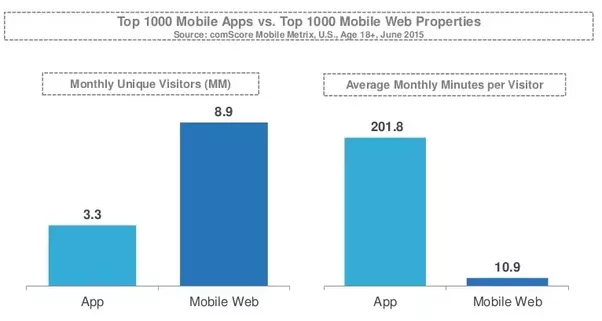
\includegraphics[scale=.7]{im1.png}
		\vspace{.1 cm}
    \caption{App and Mobile web usage}
	\end{center}
\end{figure}
\item The Web reaches wider audiences than apps. But apps dominate in time spent. So there is need of something that combines the best experiences of the web and the app. A new architecture is coming that will help to combine the best experiences of the web and the app and may finally provide the solution to building apps and websites that are fast and reliable. With Progressive Web Apps, Google has seen engagement levels of websites approach nearly that of native apps.In a nut shell, progressive Web apps start out as tabs in Chrome and become progressively more “app” like the more people use them, to the point where they can be pinned on the home screen of a phone or in the app drawer and have access to app-like properties such as notifications and offline use. Progressive Web apps are linkable with an URL, fully responsive and secure.


\begin{enumerate}
\end{enumerate}




 

\chapter{Comparative Study}
\section{Native Applications:}
 
\item
Native applications have codes that are devised specifically for a particular platform, namely Android, iOS and so on. Cross-platform codes are not possible with native apps as the codes written for one platform cannot be used in another. You may use the latest APIs, but you cannot use one platform’s code on another one. A native app would always feel right for the user because it has a mature ecosystem containing all the specific guidelines used for the OS it is developed for; ranging from swipes, app defines gestures to centrally aligned headers for iOS and left aligned headers for Android. This makes it easier for the user.
\section{Web Apps:}
\item 
Mobile web applications require web browsers to function and they are developed using HTML ,CSS and JavaScript. The program will be stored on a remote server and shows itself when the user asks for it. It is not necessary for web apps to have native codes and they can function on any operating system.
\section{Hybrid Apps:}
\item When smartphones were first released into the market, the war between native and web applications took shape and form, but along with the spoils of the war, another category was created – hybrid apps. If you want to get an app out the door as soon as possible and save time and money on developing the app, then you need hybrid apps. Hybrid app development is cross-platform app development and only one source code is used; this would be upgraded and updated to suit the purpose. Thus it combines the benefits of both native apps and web apps.
\section{Comparative factors:}
\begin{itemize}
    \item \textbf{Code Portability:}
You can not port native apps from one platform to another. With web apps, you can have a single code base for any major mobile platform. This is not 100 percent portable and sometimes developers are faced with portability issues. For hybrid apps, you can reuse many of the apps from one platform to another.
    \item \textbf{Local Storage, Offline Capability:}
Offline apps would function even when your user is not online. There is no need for the internet connection to beconstant. Local storage that retains web app data is possible with web apps, and thus it would be ideal to use web apps if you are looking for offline storage of 5MB at a time. With hybrid apps, users cannot enjoy the offline mode as much as they would want. With native apps, it would be possible for users to enjoy the capabilities of offline capability.
    \item \textbf{Monetization:}
Every app developer seeks to come up with a ground- breaking concept when they release their app to the app store. They all expect it to bring in phenomenal success in terms of money. The possibility of monetization with native and hybrid apps would be much higher compared to web apps. The downside for native and hybrid apps is that the app store takes a percentage of all sales that you make. Whereas, for web apps, there are no commissions.
    \item \textbf{Cost:}
Native apps often cost more to develop because they ask for specific language and tooling ecosystems, apart from the customization of code. Cost is often dependant on a number of factors and sometimes even the skill of a developer which could cost more. Web app’s functionality is based on JavaScript, CSS and HTML5. Hybrid apps are least expensive of all three.
    \item \textbf{Time to Market Apps:}
App store is quite strict about the apps sold in their store and things get stricter for in app purchases. You have to submit an application and sometimes, wait for months to get their approval. The time to market for web apps is much smoother and simpler, whereas for the other two, you will have to wait.
    \item \textbf{User Experience and Interaction:}
Native app provides much better accessibility features when in a native UI. You have absolute control here. Unfortunately, web apps are hindered by the capability of a web browser. For native apps, you can actually accelerate the UI performance when you enhance the capabilities of the device hardware.
    \item \textbf{Internationalization & Localization:}
Every app development company dreams of surpassing geographical boundaries and creating software that people from anywhere can access. Internationalization & Localization for hybrid, native and web apps is excellent because the software can be designed in such a way that they can be adapted to any language without making engineering changes. These softwares can be localized by making it applicable for a particular region or language.
\end{itemize}
\chapter{Progressive Web Apps}


\item \textbfA Progressive web app combines the best experiences of the web and an app. They don't require any installation. The word 'progressive' comes from the relationship that the user builds with the app over time. The app loads quickly, even when the user is on bad networks. It can send relevant push notifications to the user and has an icon on the home screen and loads as top-level, full screen experience.

\item A progressive web app can be defined as :

\item\textbf{Reliable -} Load instantly and never show the downasaur, even in uncertain network conditions.

\item \textbf{Fast -} Respond quickly to user interactions with silky smooth animations and no janky scrolling.
\item \textbf{Engaging -} Feel like a natural app on the device, with an immersive user experience.
\item \textbf{Why build a Progressive Web App?}
\newline Building a high-quality Progressive Web App has incredible benefits, making it easy to delight your users, grow engagement and increase conversions.
\begin{itemize}
\item Worthy of being on the home screen
When the Progressive Web App criteria are met, Chrome prompts users to add the Progressive Web App to their home screen.
\item Work reliably, no matter the network conditions
Service workers enabled Konga to send 63\% less data for initial page loads, and 84\% less data to complete the first transaction!
\item Increased engagement
Web push notifications helped eXtra Electronics increase engagement by 4X. And those users spend twice as much time on the site.
\item Improved conversions
The ability to deliver an amazing user experience helped AliExpress improve conversions for new users across all browsers by 104\% and on iOS by 82\%.
\end{itemize}
\textbf{Characteristics}

There are certain characteristics that define PWAs, and that differentiate them from regular Web sites and native or cross-platform mobile apps. The main differentiator between a regular Web site and a PWA is the added functionality and User Experience (UX) the latter provides. Where a regular Web site requires the user to open a browser, type in a URL and wait for all content to be downloaded on every visit, effectively preventing an offline experience, a PWA only requires these steps for the first visit. After a home screen installation, all necessary static files, including HTML, CSS, JavaScript, images and fonts for the Web site, are now stored on the user’s phone, ready to be used offline. All dynamic data can be cached for offline (or low-connectivity) use, and re-fetched when needed, e.g. when new data is available and the phone is on a decent network connection.
Where a regular Web site would be wrapped in a browser (e.g. Chrome Android) with visible browser artefacts (such as address bar and menus), a PWA will similarly run in a browser instance, but without those artefacts. Thus, a PWA will look similar to a regular app. If a PWA is styled correctly, following the design guidelines of each mobile platform, telling apart a regular native or cross-platform app and a PWA from the appearance would be challenging.


\chapter{Core building blocks of Progressive web app}
\section{Application shell}
\item An Application shell (or app shell) architecture is one way to build a Progressive Web App that reliably and instantly loads on your users' screens, similar to what you see in native applications.


The app "shell" is the minimal HTML, CSS and JavaScript required to power the user interface and when cached offline can ensure instant, reliably good performance to users on repeat visits. This means the application shell is not loaded from the network every time the user visits. Only the necessary content is needed from the network.
\begin{figure}[h!]
		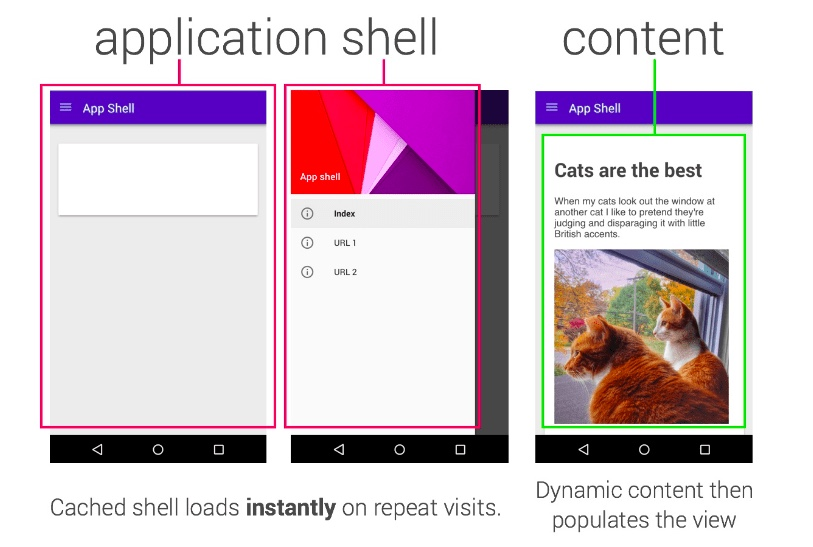
\includegraphics[scale=.56]{apshell.jpeg}
    \caption{App shell}
\end{figure}
\newline
\newline
For single-page applications with JavaScript-heavy architectures, an application shell is a go-to approach. This approach relies on aggressively caching the shell (using a service worker) to get the application running. Next, the dynamic content loads for each page using JavaScript. An app shell is useful for getting some initial HTML to the screen fast without a network.

\subsection{When to use app shell model}
\itemBuilding A PWA does not mean starting from scratch. If you are building a modern single-page app, then you are probably using something similar to an app shell already whether you call it that or not. The details might vary a bit depending upon which libraries or frameworks you are using, but the concept itself is framework agnostic.

An application shell architecture makes the most sense for apps and sites with relatively unchanging navigation but changing content. A number of modern JavaScript frameworks and libraries already encourage splitting your application logic from its content, making this architecture more straightforward to apply. For a certain class of websites that only have static content you can still follow the same model but the site is 100% app shell.
\subsection{Benefits}
\item

The benefits of an app shell architecture with a service worker include:
\begin{itemize}
    \item \textbf{Reliable performance that is consistently fast}. Repeat visits are extremely quick. Static assets and the UI (e.g. HTML, JavaScript, images and CSS) are cached on the first visit so that they load instantly on repeat visits. Content may be cached on the first visit, but is typically loaded when it is needed.
    \item \textbf{Native-like interactions}. By adopting the app shell model, you can create experiences with instant, native-application-like navigation and interactions, complete with offline support.
    \item \textbf{Economical use of data}. Design for minimal data usage and be judicious in what you cache because listing files that are non-essential (large images that are not shown on every page, for instance) result in browsers downloading more data than is strictly necessary. Even though data is relatively cheap in western countries, this is not the case in emerging markets where connectivity is expensive and data is costly.
\end{itemize}


\subsection{Requirements}
\item The app shell should ideally:
\begin{itemize}
    \item Load fast
    \item Use as little data as possible
    \item Use static assets from a local cache
    \item Separate content from navigation
    \item Retrieve and display page-specific content (HTML, JSON, etc.)
    \item Optionally, cache dynamic content
\end{itemize}

\section{Service workers}
\item A service worker is a script that your browser runs in the background, separate from a web page, opening the door to features that don't need a web page or user interaction. Today, they already include features like push notifications and background sync. In the future, service workers might support other things like periodic sync or geofencing. The core feature discussed in this tutorial is the ability to intercept and handle network requests, including programmatically managing a cache of responses.

The reason this is such an exciting API is that it allows you to support offline experiences, giving developers complete control over the experience.

\item Things to note about a service worker:
\begin{itemize}
    \item It's a JavaScript Worker, so it can't access the DOM directly. Instead, a service worker can communicate with the pages it controls by responding to messages sent via the postMessage interface, and those pages can manipulate the DOM if needed.
    \item Service worker is a programmable network proxy, allowing you to control how network requests from your page are handled.
    \item It's terminated when not in use, and restarted when it's next needed, so you cannot rely on global state within a service worker's onfetch and onmessage handlers. If there is information that you need to persist and reuse across restarts, service workers do have access to the IndexedDB API.
    \item Service workers make extensive use of promises, so if you're new to promises, then you should stop reading this and check out Promises, an introduction.
\end{itemize}
\subsection{The service worker life cycle}
\item A service worker has a lifecycle that is completely separate from your web page.

To install a service worker for your site, you need to register it, which you do in your page's JavaScript. Registering a service worker will cause the browser to start the service worker install step in the background.

Typically during the install step, you'll want to cache some static assets. If all the files are cached successfully, then the service worker becomes installed. If any of the files fail to download and cache, then the install step will fail and the service worker won't activate (i.e. won't be installed). If that happens, don't worry, it'll try again next time. But that means if it does install, you know you've got those static assets in the cache.

When installed, the activation step will follow and this is a great opportunity for handling any management of old caches, which we'll cover during the service worker update section.

After the activation step, the service worker will control all pages that fall under its scope, though the page that registered the service worker for the first time won't be controlled until it's loaded again. Once a service worker is in control, it will be in one of two states: either the service worker will be terminated to save memory, or it will handle fetch and message events that occur when a network request or message is made from your page.
\newpage
\begin{figure}[h]
		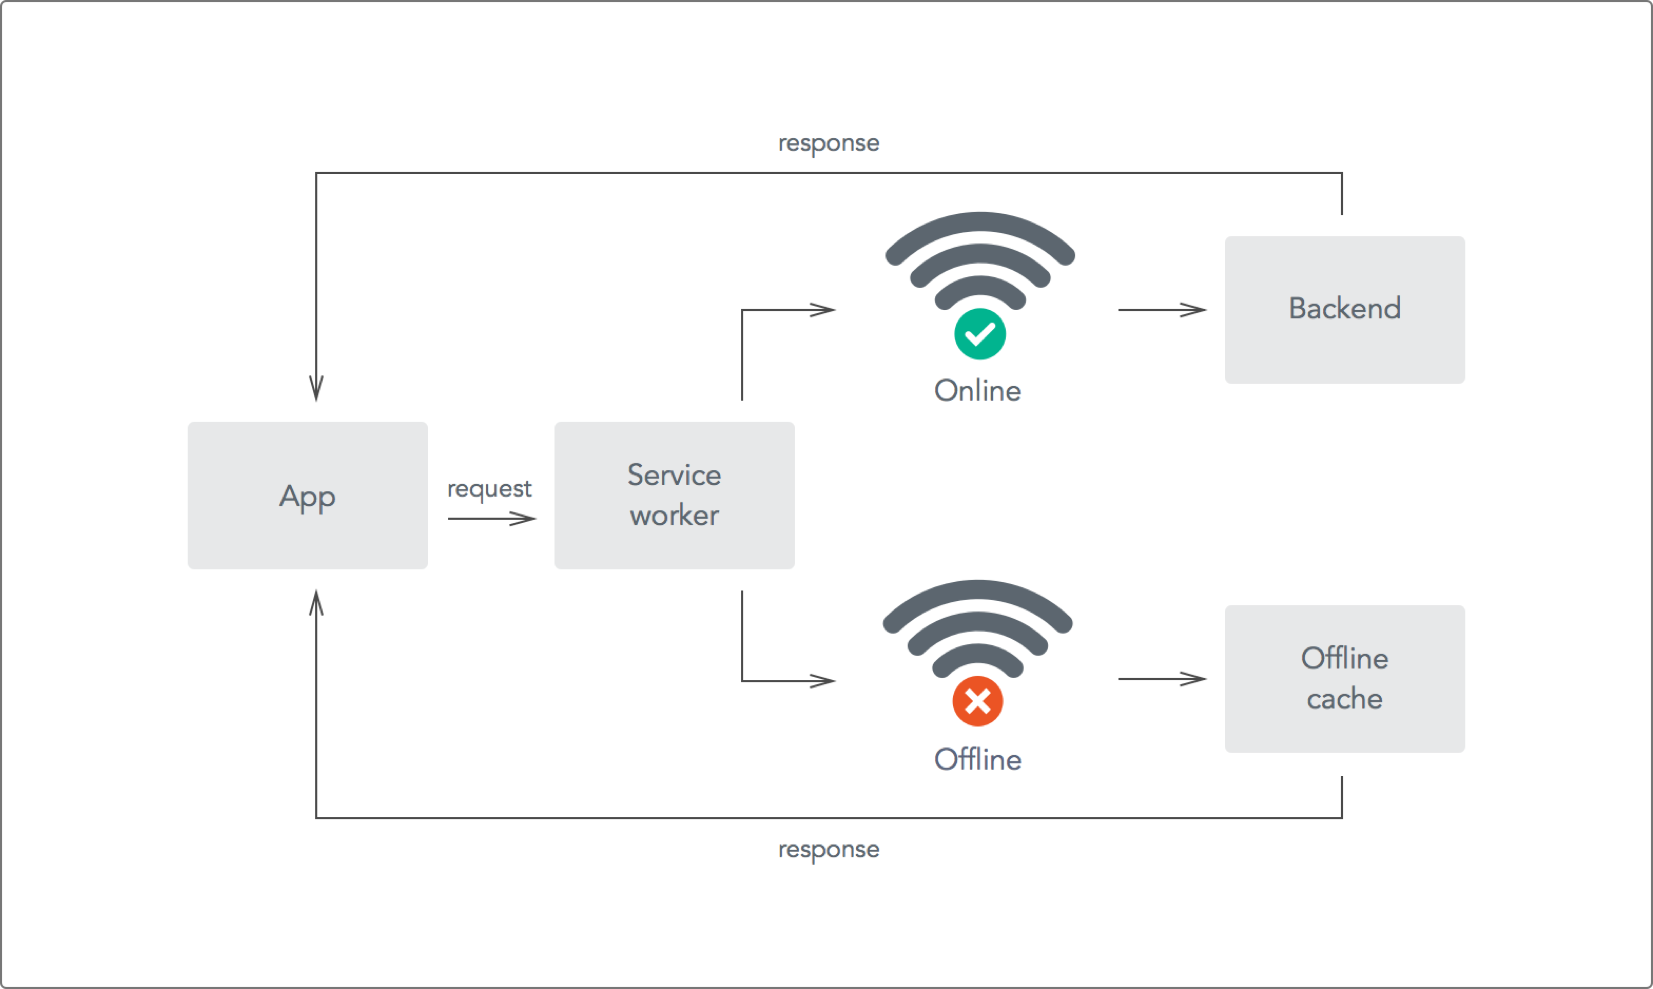
\includegraphics[scale=.56]{P1.png}
	
    \caption{Life cycle}
\end{figure}
\subsection{Prerequisites}
\begin{itemize}
    \item \textbf{Browser support}

Browser options are growing. Service workers are supported by Chrome, Firefox and Opera. Microsoft Edge is now showing public support. Even Safari has dropped hints of future development. You can follow the progress of all the browsers at Jake Archibald's is Serviceworker ready site.

\item \textbf{You need HTTPS}

During development you'll be able to use service worker through localhost, but to deploy it on a site you'll need to have HTTPS setup on your server.

Using service worker you can hijack connections, fabricate, and filter responses. Powerful stuff. While you would use these powers for good, a man-in-the-middle might not. To avoid this, you can only register service workers on pages served over HTTPS, so we know the service worker the browser receives hasn't been tampered with during its journey through the network.
\end{itemize}
\subsection{Register a service worker}
\item To install a service worker you need to kick start the process by registering it in your page. This tells the browser where your service worker JavaScript file lives.
\begin{figure}[h]
		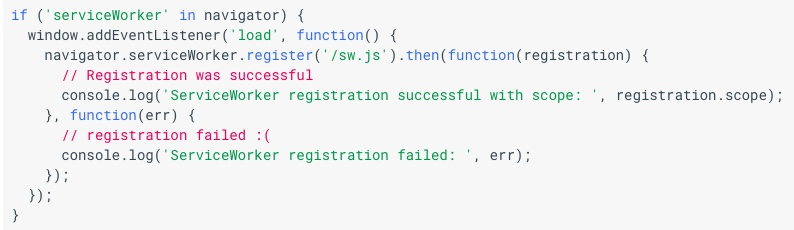
\includegraphics[scale=.6]{s1.jpeg}
	
    
\end{figure}
\item This code checks to see if the service worker API is available, and if it is, the service worker at /sw.js is registered once the page is loaded.

You can call register() every time a page loads without concern; the browser will figure out if the service worker is already registered or not and handle it accordingly.

One subtlety with the register() method is the location of the service worker file. You'll notice in this case that the service worker file is at the root of the domain. This means that the service worker's scope will be the entire origin. In other words, this service worker will receive fetch events for everything on this domain. If we register the service worker file at /example/sw.js, then the service worker would only see fetch events for pages whose URL starts with /example/ (i.e. /example/page1/, /example/page2/).
\subsection{Subsequent visits}
\item When a service worker is registered, it goes through the install and activate lifecycle events. Once a service worker is activated, it can handle fetch events for any subsequent visits to your web app. The service worker starts before the request for any pages under its scope is made, which makes sense when you think about it. If the existing service worker weren't already running prior to visiting a page, it wouldn't have a chance to fulfill fetch events for navigation requests.

So once there's an active service worker, it doesn't matter when you call navigator.serviceWorker.register(), or in fact, whether you call it at all. Unless you change the URL of the service worker script, navigator.serviceWorker.register() is effectively a no-op during subsequent visits. When it's called is irrelevant.
\section{App manifest}
\item The web app manifest is a simple JSON file that tells the browser about your web application and how it should behave when 'installed' on the user's mobile device or desktop. Having a manifest is required by Chrome to show the Add to Home Screen prompt.

A typical manifest file includes information about the app name, icons it should use, the start url it should start at when launched, and more.
\item A complete manifest.json file for a progressive web app
\begin{figure}[h]
		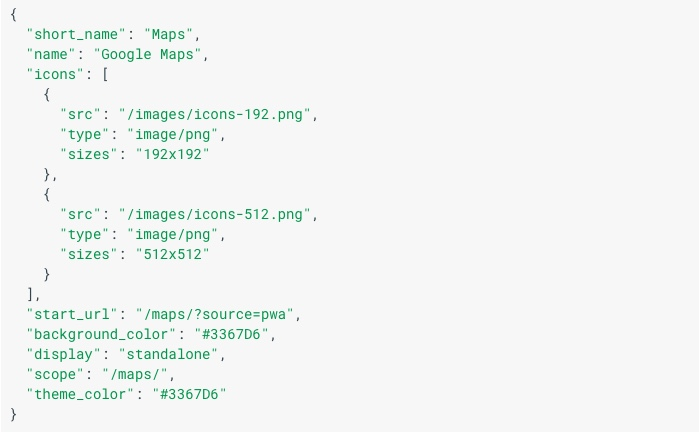
\includegraphics[scale=.7]{s2.jpeg}
	
    
\end{figure}

\chapter{Features of Progressive web apps}
\section{Offline Storage}
\item Internet connections can be flakey or non-existent on the go, which is why offline support and reliable performance are common features in progressive web apps. Even in perfect wireless environments, judicious use of caching and other storage techniques can substantially improve the user experience. In this post, we’ll summarize some ideas around offline data storage for PWAs — think JSON payloads, images and general static data required to provide a meaningful experience offline.
\item General recommendation for storing data offline:
\begin{itemize}
    \item For the network resources necessary to load your app while offline, use the Cache API (part of service workers).
    \item For all other data, use IndexedDB (with a promises wrapper).
\end{itemize}
\item Both APIs are asynchronous (IndexedDB is event based and the Cache API is Promise based). They also work with web workers, window and service workers. IndexedDB is available everywhere. Service Workers (and the Cache API) are now available in Chrome, Firefox, Opera and are in development for Edge. Promise wrappers for IndexedDB hide some of the powerful but also complex machinery (e.g. transactions, schema versioning) that comes with the IndexedDB library. IndexedDB will support observers, which allow easy synchronization between tabs.
\item For PWAs, you can cache static resources, composing your application shell (JS/CSS/HTML files) using the Cache API and fill in the offline page data from IndexedDB. Debugging support for IndexedDB is now available in Chrome (Application tab), Opera, Firefox (Storage Inspector) and Safari (see the Storage tab).

\section{Offline Access}
\item Service workers can use the Cache interface to cache an application's assets. A service worker script can implement a number of caching strategies, allowing fine tuning of an app's offline and low-connectivity performance.

The Cache interface's storage is controlled programmatically and is independent of the browser's HTTP cache. Unlike the browser's HTTP cache, the Cache interface's storage is available offline. The service worker can use this to enable offline support in browsers.

Service workers can also use IndexedDB to store data locally. This enables new features such as capturing user actions while offline and delivering them once connectivity returns.
\item \textbf{Implementation}
\begin{enumerate}
    \item Register a service worker (for first time app visits, this triggers service worker installation).
    \item On service worker installation, cache the app's static assets (generally the minimum HTML, CSS, and JS that the app needs to open).
    \item Have the service worker listen for resource fetches. When a resource is fetched, have the service worker attempt to find the resource in the cache before going to the network.
    \item If a resource must be retrieved from the network, have the service worker cache a copy of the resource so that it can be retrieved from the cache in the future.
\end{enumerate}
\newpage  \section{Push Notifications}
\subsection{What are Push Notifications?}
\item A notification is a message that pops up on the user's device. Notifications can be triggered locally by an open application, or they can be "pushed" from the server to the user even when the app is not running. They allow your users to opt-in to timely updates and allow you to effectively re-engage users with customized content.

Push Notifications are assembled using two APIs: the Notifications API and the Push API. The Notifications API lets the app display system notifications to the user. The Push API allows a service worker to handle Push Messages from a server, even while the app is not active.

The Notification and Push API's are built on top of the Service Worker API, which responds to push message events in the background and relays them to your application.

\subsection{Understanding Push Notifications on the web}\item Push notifications let your app extend beyond the browser, and are an incredibly powerful way to engage with the user. They can do simple things, such as alert the user to an important event, display an icon and a small piece of text that the user can then click to open up your site. You can also integrate action buttons in the notification so that the user can interact with your site or application without needing to go back to your web page.

There are several pieces that come together to make push notifications work. Browsers that support web push each implement their own push service, which is a system for processing messages and routing them to the correct clients. Push messages destined to become notifications are sent from a server directly to the push service, and contain the information necessary for the push service to send it to the right client and wake up the correct service worker. The section on the Push API describes this process in detail.

When it receives a message, the service worker wakes up just long enough to display the notification and then goes back to sleep. Because notifications are paired with a service worker, the service worker can listen for notification interactions in the background without using resources. When the user interacts with the notification, by clicking or closing it, the service worker wakes up for a brief time to handle the interaction before going back to sleep.
\item \textbf{Notifications API }
\item The Notifications API lets us display notifications to the user. It is incredibly powerful and simple to use. Where possible, it uses the same mechanisms a native app would use, giving a completely native look and feel.
\item We can split the Notifications API into two core areas (these are non-technical and are not part of the spec). The Invocation API * controls how to make your notification appear, including styling and vibration. We create (or invoke) the notification from the page (or from the server, in the case of push notifications). The Interaction API* controls what happens when the user engages with the notification. User interaction is handled in the service worker.
\item \textbf{Push API }
\item Push messaging lets developers engage users by providing timely and customized content outside the context of the web page. It is one of the most critical APIs to come to the web, giving users the ability to engage with web experiences even when the browser is closed, without the need for a native app install.

\item \textbf{Process}
\item On the client:
\begin{enumerate}
    \item Subscribe to the push service
    \item Send the subscription object to the server
\end{enumerate}
On the server:
\begin{enumerate}
    \item Generate the data that we want to send to the user
    \item Encrypt the data with the user public key
    \item Send the data to the endpoint URL with a payload of encrypted data.
\end{enumerate}

The message is routed to the user's device. This wakes up the browser, which finds the correct service worker and invokes a "push" event. Now, on the client:
\begin{enumerate}
    \item Receive the message data (if there is any) in the "push" event
    \item Perform some custom logic in the push event
    \item Show a notification
\end{enumerate}
\newline
\newline
\item
\item 
\begin{figure}[h]
		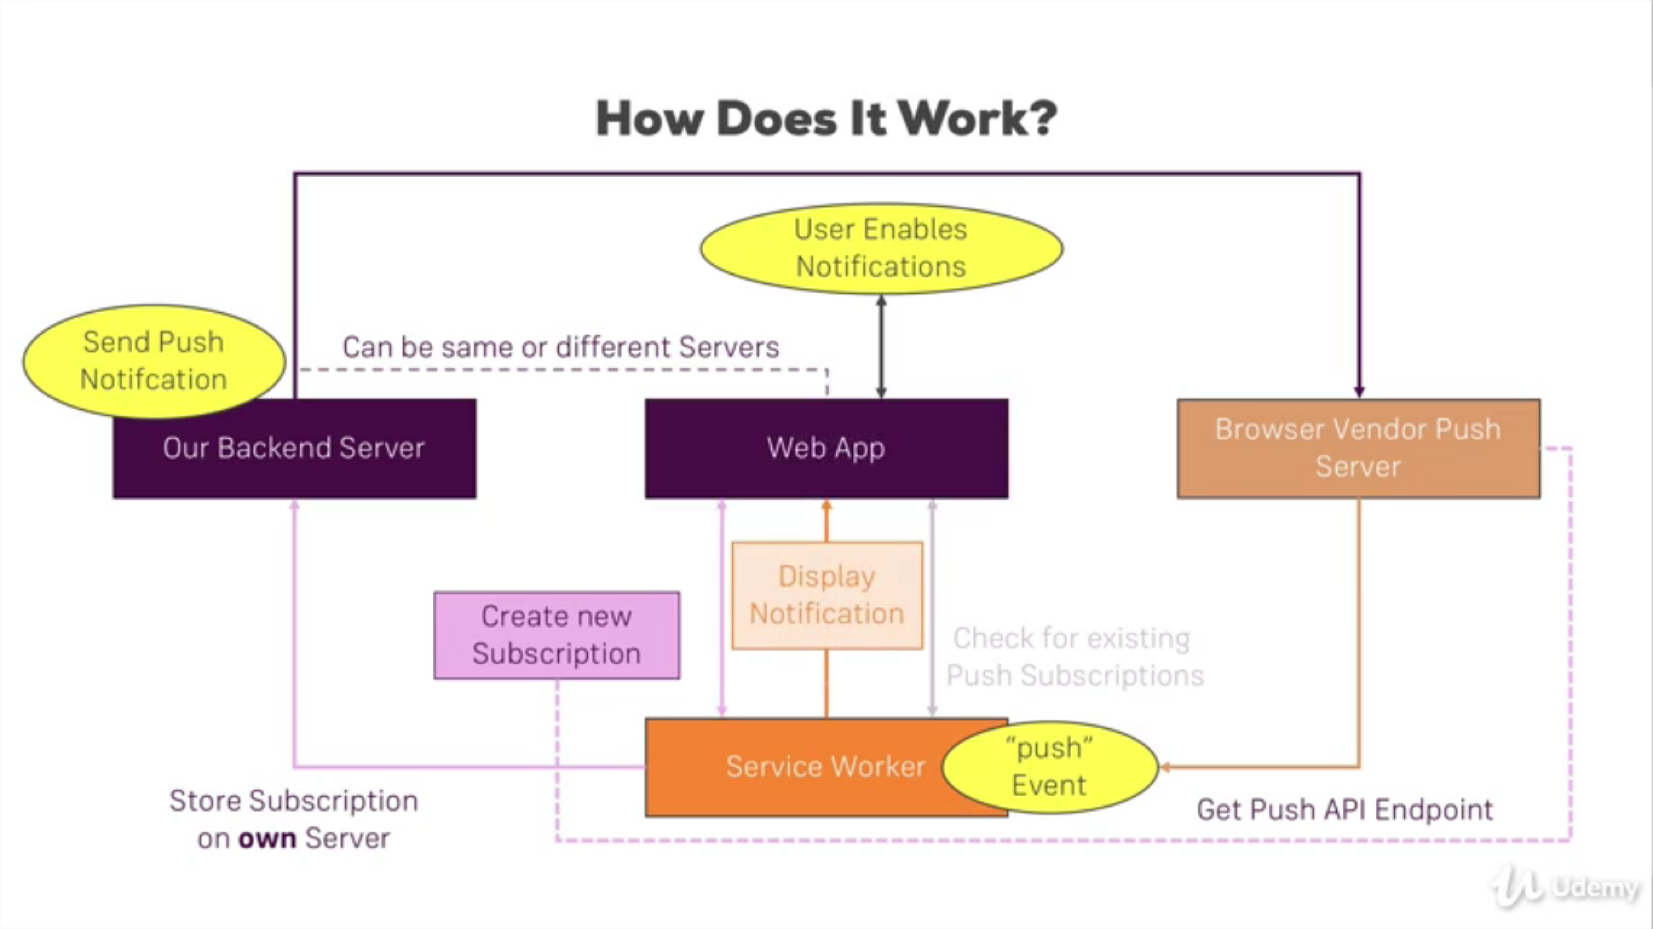
\includegraphics[scale=.6]{ss3.png}
		\caption{Working of push notification}
	
    
\end{figure}

\newpage
\section{Add to home screen}
\item Add to Home Screen, sometimes referred to as the web app install prompt, makes it easy for users to install your Progressive Web App on their mobile or desktop device. After the user accepts the prompt, your PWA will be added to their launcher, and it will run like any other installed app.

\item Chrome handles most of the heavy lifting for you:
\begin{itemize}
    \item On mobile, Chrome will generate a WebAPK, creating an even more integrated experience for your users.
    \item On desktop, your app will installed, and run in an app window.
\end{itemize}
\newline
\item \textbf{Criteria}
\item In order for a user to be able to install your Progressive Web App, it needs to meet the following criteria:
\begin{itemize}
    \item The web app is not already installed
    \item Meets a user engagement heuristic (currently, the user has interacted with the domain for at least 30 seconds)
    \item Includes a web app manifest that includes:
    \begin{itemize}
        \item short\_name or name
        \item icons must include a 192px and a 512px sized icons
        \item start\_url
        \item display must be one of: fullscreen, standalone, or minimal-ui
    \end{itemize}
    \item Served over HTTPS (required for service workers)
    \item Has registered a service worker with a fetch event handler

\end{itemize}
\item 
\item \textbf{Show the Add to Home Screen Dialogue}
\item In order to show the Add to Home Screen dialog, you need to:
\begin{enumerate}
    \item Listen for the beforeinstallprompt event
    \item Notify the user your app can be installed with a button or other element that will generate a user gesture event.
    \item Show the prompt by calling prompt() on the saved beforeinstallprompt event.
\end{enumerate}

\begin{figure}[h!]
        \centering
		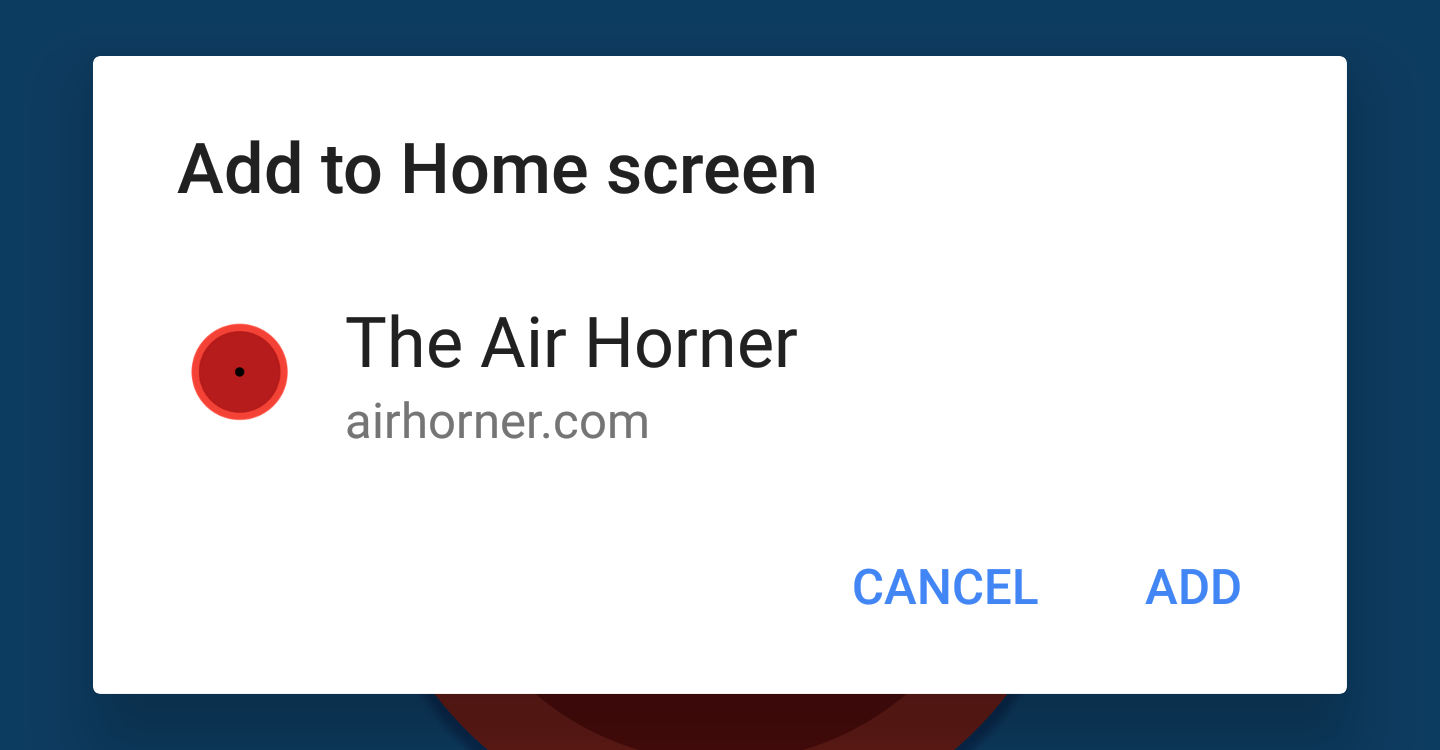
\includegraphics[scale=.25]{ss4.png}
		\caption{Add to Home Screen prompt}
\end{figure}



\newpage
\chapter{Security}
\section{Encrypting Data In Transit}
\item One of the most critical security features, and one that is required for many modern APIs and progressive web apps is HTTPS, sometimes referred to as secure HTTP.

Some people mistakenly believe that the only sites that need HTTPS are sites that handle some level of sensitive communication, like personal or financial data. But this isn't true. Every site should be using HTTPS, HTTPS helps to prevents people from listening into what's crossing the wire, and helps prevent it from being tampered with while in transit. 
\item \textbf{Why HTTPS}
\begin{itemize}
    \item Intruders both malignant and benign exploit every unprotected resource between your websites and users.
    \iem Many intruders look at aggregate behaviors to identify your users.
    \item HTTPS doesn't just block misuse of your website. It's also a requirement for many cutting-edge features and an enabling technology for app-like capabilities such as service workers.
\end{itemize}
\item \textbf{Enabling HTTPS}
\begin{itemize}
    \item Create a 2048-bit RSA public/private key pair.
    \item Generate a certificate signing request (CSR) that embeds your public key.
    \item Share your CSR with your Certificate Authority (CA) to receive a final certificate or a certificate chain.
    \item Install your final certificate in a non-web-accessible place such as /etc/ssl (Linux and Unix) or wherever IIS requires it (Windows).
\end{itemize}

\section{Content Security Policy}
\item Cross-site scripting (XSS) attacks, for example, bypass the same origin policy by tricking a site into delivering malicious code along with the intended content. This is a huge problem, as browsers trust all of the code that shows up on a page as being legitimately part of that page's security origin. The XSS Cheat Sheet is an old but representative cross-section of the methods an attacker might use to violate this trust by injecting malicious code. If an attacker successfully injects any code at all, it's pretty much game over: user session data is compromised and information that should be kept secret is exfiltrated to The Bad Guys. We'd obviously like to prevent that if possible.
\item This overview highlights a defense that can significantly reduce the risk and impact of XSS attacks in modern browsers: \textbf{Content Security Policy (CSP)}.
\begin{itemize}
    \item Use whitelists to tell the client what's allowed and what isn't.
    \item Learn what directives are available.
    \item Learn the keywords they take.
    \item Inline code and eval() are considered harmful.
    \item Report policy violations to your server before enforcing them
\end{itemize}

\newpage \section{Preventing Mixed Content}
\item \textbf{What is Mixed Content ?}
\item Mixed content occurs when initial HTML is loaded over a secure HTTPS connection, but other resources (such as images, videos, stylesheets, scripts) are loaded over an insecure HTTP connection. This is called mixed content because both HTTP and HTTPS content are being loaded to display the same page, and the initial request was secure over HTTPS. Modern browsers display warnings about this type of content to indicate to the user that this page contains insecure resources.

\item \textbf{Browser behavior with mixed content}
\item Modern browsers follow mixed content specification, which defines optionally blockable content and blockable content categories.

From the spec, a resource qualifies as optionally blockable content "when the risk of allowing its usage as mixed content is outweighed by the risk of breaking significant portions of the web"; this is a subset of the passive mixed content category. At the time of this writing, images, video, and audio resources, as well as prefetched links, are the only resource types included in optionally blockable content. This category is likely to get smaller as time goes on.

All content that is not optionally blockable is considered blockable, and is blocked by the browser.

\item \textbf{Finding Mixed Content}
\begin{itemize}
    \item Finding mixed content by visiting site

    When visiting an HTTPS page in Google Chrome, the browser alerts you to mixed content as errors and warnings in the JavaScript console.

    To view these alerts, go to our passive mixed content or active mixed content sample page and open the Chrome JavaScript console.You can open the console either from the View menu: View $\rightarrow$ Developer $\rightarrow$ JavaScript Console, or by right-clicking the page, selecting Inspect Element, and then selecting Console.
    \newline 
    \item Finding mixed content in source code

    You can search for mixed content directly in your source code. Search for http:// in your source and look for tags that include HTTP URL attributes.\newline
    If you have a list of HTTP URLs from Chrome mixed content errors and warnings, you can also search for these complete URLs in your source to find where they are included in your site.
\end{itemize}
\item \textbf{Fixing mixed content}
\begin{itemize}
    \item \textbf{Step 1}

Check that the URL is available over HTTPS by opening a new tab in your browser, entering the URL in the address bar, and changing http:// to https://

If the resource displayed is the same over HTTP and HTTPS, everything is OK. Proceed to Step 2.
    \item \textbf{Step 2}

Change the URL from http:// to https://, save the source file, and redeploy the updated file if necessary.

    \item \textbf{Step 3}

View the page where you found the error originally and verify that the error no longer appears.
\end{itemize}

\item \textbf{Blocking all mixed content}
\item Not all browsers support the upgrade-insecure-requests directive, so an alternative for protecting users is the block-all-mixed-content CSP directive. This directive instructs the browser to never load mixed content; all mixed content resource requests are blocked, including both active and passive mixed content. This option also cascades into <iframe> documents, ensuring the entire page is mixed content free.
\item The downside of using block-all-mixed-content is, perhaps obviously, that all content is blocked. This is a security improvement, but it means that these resources are no longer available on the page. This might break features and content that your users expect to be available.
\chapter{Case Studies}
\section{BookMyShow}
\item 
BookMyShow’s new Progressive Web App drives an 80\% increase in conversions


BookMyShow is India’s largest ticketing firm, with 50+ million monthly visitors. They developed an improved version of their mobile website using a Progressive Web App (PWA), delivering an 80+\% increase in conversions, which means more users purchasing tickets.
\item \textbf{Challenges}

BookMyShow has a growing mobile audience. Over 85\% of transactions happen on mobile, and the company’s mobile web traffic recently overtook their desktop web traffic. Even with this growth in traffic, the company still encountered high bounce rates because their mobile website's load speed and user experience weren’t optimal.

Their native app also posed problems as it required heavy data and memory usage to be effective. “People were using the native app and were happy with it, but their main concerns were the data usage and the memory it consumes,” says Anish Tripathi, Vice President of Design. “And if they uninstalled the app and tried using the mobile browser, it didn’t work the same way.”

\item \textbf{Solution}

Knowing that speed and efficiency are key to a good ticket-buying experience, BookMyShow launched a PWA to deliver the best mobile web experience possible to the majority of their users. A PWA would provide a smooth, seamless movie- booking experience that would optimize speed and remove data constraints for existing customers, without sacrificing the user experience.

The shift to a PWA also gave BookMyShow the opportunity to simultaneously migrate away from their PHP backend stack, which involved redoing some core development work. They adopted cutting-edge solutions and built a truly powerful, technically-advanced web app that provides users with fast, reliable, and engaging experiences just like the native app.

The PWA is optimized for speed. The goal for the app—which took only 10 months to build—was created to enable checkout within 30 seconds. They were also excited to use the “add to home screen” feature to provide a native-app like experience. Their PWA application is only about 440KB — 54 times smaller than the Android app and 180 times smaller than the iOS app. BookMyShow also took advantage of service workers to deliver reliable performance on slow or unreliable networks. Data consumption is also substantially lower, thanks to optimization. When a user asks for a particular page, only assets required for that page are loaded, conserving data. On 2G networks, the initial load time is just 4 seconds. Even for personalized movie suggestions, the PWA takes less than 2.94 seconds in subsequent loads. All of these changes resulted in an 80+\% increase in conversion rates, a huge difference in BookMyShow’s bottom line.
\begin{figure}[h!]
        \centering
		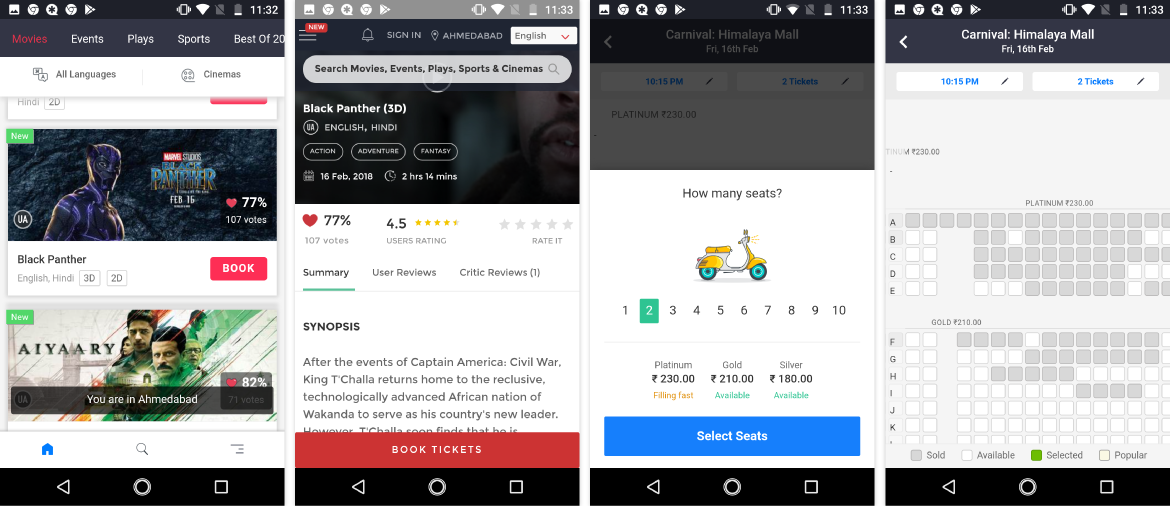
\includegraphics[scale=.35]{ss5.png}
		\caption{PWA of BookMyShow}
\end{figure}
\newpage
\section{Ola}
\item Ola is the leading cab aggregator in India, with a relentless mission to drive mobility for a billion Indians. The company reaches over 100 Indian cities with a network of about 600K driver-partners. As one of India’s most highly valued startups, Ola completes more than a million daily rides, fighting for the lion’s share of the country’s estimated 300 million daily taxi trips.
\item \textbf{Challenges}

Tier 2 and Tier 3 cities (cities with populations of 20,000 to 99,000) pose unique challenges and opportunities for Ola. Demand for sustainable, reliable transport services is growing rapidly and is eagerly anticipated in these areas. People in these cities often deal with intermittent cellular connectivity and have low-end smartphones with low memory and slow processors. These users are less apt to download and store native apps on their smartphones because native apps require high data usage and take up a lot of space —the Ola Android app is a 60MB download and the iOS app is 100M. It was clear that Ola needed a different way to reach these users.

The mobile web presented a perfect solution. It offers easy discovery and low friction—users just click a link instead of downloading an app. Other advantages include push notifications, and the “Add to Home screen“ user prompt. As Dipika Kapadia, Ola’s head of consumer web products notes, “Apps have many advantages but must be developed for different operating systems, while a single site is good for any browser.”

\item \textbf{Solution}

Ola built their mobile website as a Progressive Web App (PWA). Using just 200KB of data to install, the PWA is at least 300X smaller than downloading the Android app and 500X smaller than downloading their iOS app. Repeat visits use as little as 10KB. This low data consumption translates into a 3.4-second first visit and less than a second for repeat visits on 2G and 3G networks—an ideal solution for millions of Indians.
Ola also noticed that 20\% of users who book using their PWA had previously uninstalled their app. By reducing the amount of storage space needed, the PWA allowed them to effectively re-engage with their previous app users.
The PWA is helping Ola reach a broader set of users in new cities. They’ve seen mobile traffic from Tier 2 and Tier 3 cities grow by 68\%. Since launch, conversion rates on the PWA have been the same as their native app in Tier 2 cities, and for Tier 3 cities, conversion rates are 30\% higher on the PWA.
\begin{figure}[t]
        \centering
		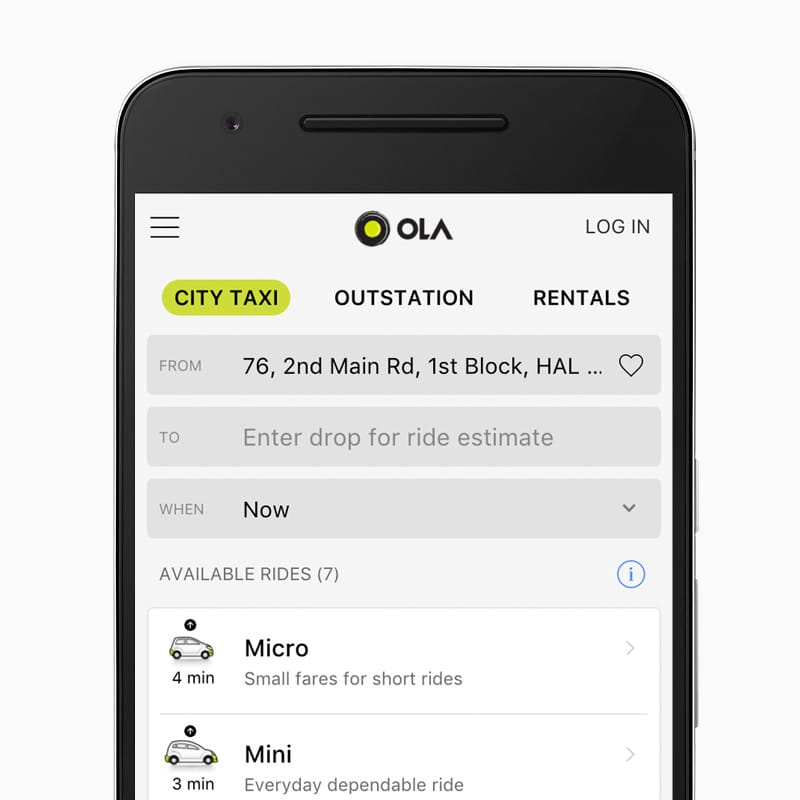
\includegraphics[scale=.3]{ss5.jpg}
		\caption{PWA of Ola}
\end{figure}


\chapter{Technological Prospects and Limitations}
A substantial developer-oriented effort was presented du- ring Google I/O 2017 [80], where Osmani showcased a technical baseline for testing JavaScript frameworks against PWA criteria. The baseline, named HNPWA , aims at helping developers choose a JavaScript front-end framework for building PWAs. Numerous frameworks are included in the test, such as React, Preact, Svelte, Vue.js and Angu- lar. All the tests’ code-bases are open-source, and tests using new frameworks and approaches can be added to the HNPWA Web site for others to learn from.
\item 
\newline
For PWAs, access to device and platform APIs is still con- strained to those APIs supported by the users’ browsers. This is one of the major limitations of the PWA approach when compared to native or cross-platform development where all, or most, open device APIs are exposed to the developer through the native SDKs or similar abstractions. Somewhat reassuring, the Google Chrome team added 215 new APIs in the last year alone, so progress to bridge that gap is undoubtedly improving. Nevertheless, with the inherent future introduction of new mobile platform features, PWAs’ access to them is still limited until an HTML/JavaScript specification has been formalized by W3C and (or at least) is implemented by browser vendors. Fragmentation of plat- forms, operating systems versions and browser- and device capabilities do not help the Web move towards unification.
Interestingly, even concerning programming languages the Web might see further fragmentation. An notable technology, slowly gaining traction in the industry, is WebAs- sembly (wasm), a format and enabler for writing Web applications using other languages than JavaScript. This may open the porting of software, specifically of games, which traditionally only ran as native desktop applications. For Webapps and PWAs, support for multiple languages might introduce new developers to the platform, which could lead to further adoption and proliferation of such apps.




\chapter{Status Quo of PWA adoption}
 During Google’s developer conference, Google I/O 2017, a number of Progressive Web Apps initiatives were presen- ted both on-stage and as mentions. Large companies and key players in the mobile-Web space have already started con- verting their existing Web apps to PWAs with great success. This includes the before mentioned Twitter and OLA, both leading companies within their fields. The companies also revealed statistics about app sizes and reported increased usage after PWA adoption.
 \item
\newline Other notable companies working on PWAs include For- bes, Financial Times, Lyft, Expedia, AliExpress, Tinder, Flipkart, and Housing.com. These companies and their pro- ducts represents different niches and markets, illustrating how PWAs can be a fit anywhere.
\item 
\newline Also during the conference, seven talks were directed towards the development of- and enthusiasm for this possible next generation of the mobile Web. PWAs were discussed in the context of mobile User Experience (UX), support by technical frameworks, performance testing and migration. Google is obviously pushing PWAs as an effort to improve the user experience of the mobile Web.


\chapter{Conclusion}
Progressive web apps have benefits for everyone involved. The user will be able to instantly install the “app” without a visit to the app store and a large download, which can be an unpleasant experience on a slow connection. Organizations can go back to developing web apps without requiring the requisite separate Android and iOS teams. They can update and “release” their app without going through the app store approval process. Releases and defect fixes can be deployed immediately. Web design elements are immediately picked up by the progressive web app.
A progressive web app is a website that combines the best experiences of the web and an app. They don't require any installation. The app loads quickly, even when the user is on bad networks. It can send relevant push notifications to the user and has an icon on the home screen and loads as top- level, full screen experience.
Application shell architectures comes with several benefits but only makes sense for some classes of applications. The model is still young and it will be worth evaluating the effort and overall performance benefits of this architecture. Progressive web apps are an interesting forward look into the future of mobile apps. It will become a key factor in the world of apps.


\newpage
\addcontentsline{toc}{chapter}{Bibliography}
\begin{thebibliography}{9}
\bibitem{item1}
{\fontsize{13pt}{8.4pt}\selectfont {Rahul Surendra Mishra} – Progressive WEBAPP : Review, 2016
      IRJET
\par}\par

\bibitem{item2}
{\fontsize{13pt}{8.4pt}\selectfont Abhi Gambhir, Gaurav Raj - Analysis of Cache in Service  
     Worker and Performance Scoring of Progressive Web 
     Application –2018 ICACCE
.\par}\par

\bibitem{item3}
{\fontsize{13pt}{8.4pt}\selectfont Dr. V. Karpagam, Padmavathe. R, Lakshana. R, Priyadharshini.S
      - Performance Enhancement of Webpage using Progressive Web
       Features –2017 (IJIRAE)
.\par}\par

\bibitem{item4}
{\fontsize{13pt}{8.4pt}\selectfont I. Malavolta, S. Ruberto, T. Soru, and V. Terragni, “End Users ’ Perception of Hybrid Mobile Apps in the Google Play Store,” in Mobile Services (MS), 2015 IEEE International Conference on, 2015.\par}\par

\bibitem{item5}
{\fontsize{13pt}{8.4pt}\selectfont A. Mhaske, A. Bhattad, P. Khamkar, and R. More, “Progressive
Web App for Educational System,” pp. 310–312, 2018.\par}\par

\bibitem{item6}
{\fontsize{13pt}{8.4pt}\selectfont Markov Danny, “Everything You Should Know About Progressive Web Apps,” tutorialzine,2016. [Online]. Available: http://tutorialzine.com/2016/09/everything-you-should-know-about-progressive- web-apps/.\par}\par

\bibitem{item7}
{\fontsize{13pt}{8.4pt}\selectfont Gaunt Matt, “Service Workers: an Introduction,” [Online]. Available: https://developers.google.com/web/fundamentals/getting-started/primers/service- workers. 2017\par}\par

\bibitem{item8}
{\fontsize{13pt}{8.4pt}\selectfont S. Dhillon and Q. H. Mahmoud, “An evaluation framework
for cross-platform mobile application development tools,” Software – Prac. and Exp., vol. 45, no. 10, pp. 1331–1357, 2015.\par}\par

\bibitem{item9}
{\fontsize{13pt}{8.4pt}\selectfont L. Delia, N. Galdamez, P. Thomas, L. Corbalan, and P. Pe- sado, “Multi-platform mobile application development analy- sis,” in Proc. IEEE 9th RCIS, 2015.\par}\par

\bibitem{item10}
{\fontsize{13pt}{8.4pt}\selectfont I. Malavolta, “Beyond Native Apps : Web Technologies to the Rescue ! ( Keynote ).” ACM Mobile!’16, Amsterdam, Netherlands, pp. 5–6, 2016.\par}\par

\bibitem{item11}
{\fontsize{13pt}{8.4pt}\selectfont S. Xanthopoulos and S. Xinogalos, “A comparative analysis of cross-platform development approaches for mobile appli- cations,” in Proc. 6th BCI. ACM, 2013.\par}\par

\bibitem{item12}
{\fontsize{13pt}{8.4pt}\selectfont A. I. Wasserman, “Software engineering issues for mobile application development,” in Proc. FSE/SDP, ser. FoSER ’10. New York, NY, USA: ACM, 2010.\par}\par

\bibitem{item13}
{\fontsize{13pt}{8.4pt}\selectfont A. Charland and B. LeRoux, “Mobile application develop- ment: Web vs. native,” Queueing Syst., vol. 9, no. 4, 2011.\par}\par

\bibitem{item14}
{\fontsize{13pt}{8.4pt}\selectfont J. C. Dagefo ̈rde, T. Reischmann, T. A. Majchrzak, and J. Ernsting, “Generating app product lines in a model-driven cross-platform development approach,” in Proc. 49th HICSS. IEEE CS, 2016.\par}\par

\bibitem{item15}
{\fontsize{13pt}{8.4pt}\selectfont Google Developers, “Progressive web app checklist,”
2017, https://developers.google.com/web/progressive-web-
apps/checklist.\par}\par

\bibitem{item16}
{\fontsize{13pt}{8.4pt}\selectfont M. Guant and P. Kinlan, “The web app manifest,” 2017,
https://developers.google.com/web/fundamentals/engage-and-
retain/web-app-manifest/.\par}\par

\bibitem{item17}
{\fontsize{13pt}{8.4pt}\selectfont A. Osmani and M. Gaunt, “Instant loading web
apps with an application shell architecture,” 2017, https://developers.google.com/web/updates/2015/11/app- shell.\par}\par

\bibitem{item18}
{\fontsize{13pt}{8.4pt}\selectfont “Lighthouse Scoring Guide | Tools for Web Developers.” [Online].
Available: https://developers.google.com/web/tools/lighthouse/scoring.\par}\par

\bibitem{item19}
{\fontsize{13pt}{8.4pt}\selectfont "Analysing pwa"| https://ionicframework.com/docs/developer-resources/progressive-web-apps/
.\par}\par

\end{thebibliography}


\end{document}
